\section{El experimento}
Para el experimento, los estudiantes de pregrado de una universidad privada de Bogotá fueron invitados a participar en un concurso en el que debían hacer una tarea corta y sencilla. Esa tarea debían presentarla en grupos de tres personas. Estos estudiantes con frecuencia enfrentan procesos similares en los que deben formar un grupo para producir un contenido. Por lo tanto, las decisiones que tomaron en el experimento eran cercanas a su cotidianidad. 

El objeto de estudio de este trabajo son las preferencias de los estudiantes para elegir con quién hacer la tarea dado que, cuando hacen la elección, únicamente observaban unas características generales y una serie de expresiones de género de sus pares.  Los participantes tomaron todas las decisiones en línea por lo que no hubo ningún tipo de interacción entre los participantes previo a la toma de decisiones.\footnote{El experimento fue desarrollado en Otree \citep{otree}. El protocolo experimental está disponible por solicitud}.

Primero, los estudiantes se inscribieron a participar en el concurso. El formulario de inscripción incluía la explicación de cada paso del concurso y las fechas de estos. Las instrucciones fueron dadas siempre en el marco del concurso sin revelar cuáles eran las decisiones objeto de estudio. Los participantes quedaban inscritos solo si completaban el formulario de inscripción (encuesta de entrada). El propósito de esta encuesta era recoger información general de los participantes e identificar las expresiones de género relevantes para este estudio. Las inscripciones estuvieron abiertas dos semanas.

Luego, los participantes fueron asignados aleatoriamente a una sección de nueve personas. Las secciones fueron aleatorizadas para asegurar balance en el género de los participantes y en las características con las que iban a ser descritos cuando sus pares eligieran el grupo. Una vez fueron asignados a las secciones, cada participante recibió un enlace en el que observaba una tarjeta de descripción para cada una de las otras ocho personas de su sección. A partir de estas tarjetas, debían decidir con quién prefería desarrollar la tarea siguiendo un proceso de votación que está explicado más a adelante. 

El proceso de votación estuvo habilitado durante una semana. Luego de esto, los participantes fueron informados sobre quiénes estaban en su grupo. A partir de ese momento, tuvieron diez días para hacer la tarea, a pesar de que hacerla tomaba entre 5 y 30 minutos. Una semana después de que los grupos mandaran la tarea del concurso, un panel de jurados eligió los grupos ganadores. Fueron premiados siete grupos, el premio más alto fue de más del doble del salario mínimo diario (por persona del grupo) y el premio más bajo fue de un tercio del salario mínimo diario, lo equivalente a tres salarios mínimos por hora (por persona del grupo). Antes de recibir los premios los participantes respondieron una breve encuesta de salida.

\subsection{La formación de grupos}
Para el proceso de elección, cada participante observaba una tarjeta de caracterización para cada una de las otras ocho personas de su sección. A partir de esa caracterización, los participantes debían organizar los ocho perfiles en el orden en el que querían que esas personas hicieran parte de su grupo para hacer la tarea. Es decir, la persona con la que más querían hacer la tarea la debían poner el primer lugar; la segunda persona con la que más querían hacer la tarea la debían poner en el segundo lugar; así, hasta organizar los ocho perfiles. De manera que la persona con que menos querían hacer la tarea, la debían poner en el último lugar.

Todo esto se hizo a través de un enlace para asegurar que los participantes no pudieran ver a las otras personas de su sección y por lo tanto, no pudieran identificar de quién se trataba. Que la decisión la tomaran a través de un enlace que recibían por correo pudo generar que consultaran su decisión con otros participantes. Esto no invalida los resultados por dos razones. Primero, porque en la realidad cuando uno debe escoger con quién trabajar, en muchas ocasiones consulta esa decisión con otros. Segundo, las características en la tarjeta hacían imposible rastrear perfectamente quién era la persona asociada a esa caracterización.

Luego, los grupos fueron formados en tres pasos a partir de las listas que presentó cada participante. Primero, para cada sección, una de las nueve personas fue elegida aleatoriamente. El primer grupo de esa sección fue conformado por esa persona que se eligió aleatoriamente y las dos primeras personas en su lista. Segundo, de las seis personas que no fueron asignadas al primer grupo, una persona fue elegida aleatoriamente. El segundo grupo fue conformado por esa segunda persona elegida aleatoriamente y las dos primeras personas en su lista, que no fueron asignadas al primer grupo. El tercer grupo fue conformado por las tres personas que no fueron asignadas ni al primer ni al segundo grupo.

Se utilizó este proceso de formación de grupos, siguiendo a \cite{beautifulorwhite2012}, porque es compatible en incentivos. Más aún, porque el pago estaba completamente determinado por el desempeño en la tarea y el pago se hizo al grupo entero.

\subsection{Las tarjetas}
Las tarjetas que describían a cada participante tenían: (i) una imagen de la vestimenta que ese participante reconoció usaría con mayor frecuencia para ir a la universidad, (ii) la habilidad que reportó como más fuerte entre matemáticas y comunicación (habla, escucha, y escritura), (iii) la aspiración que reportó más fuerte para los próximos diez años entre estabilidad familiar y comodidad económica, (iv) la edad y (v) el departamento de nacimiento (ver Figura \ref{fig:tarjeta}). Cada participante reportó estas características entre una serie de preguntas en la encuesta de inscripción. Por lo tanto, a pesar de que al momento de inscribirse los participantes sabían que luego sus pares iban a observar una caracterización de ellos, la encuesta tenía suficientes preguntas para no poder identificar \textit{a priori} cuáles de sus respuestas iban a aparecer en la tarjeta. 

\begin{figure}[htbp]
	\centering
	\caption{Ejemplo de tarjeta de caracterización}
	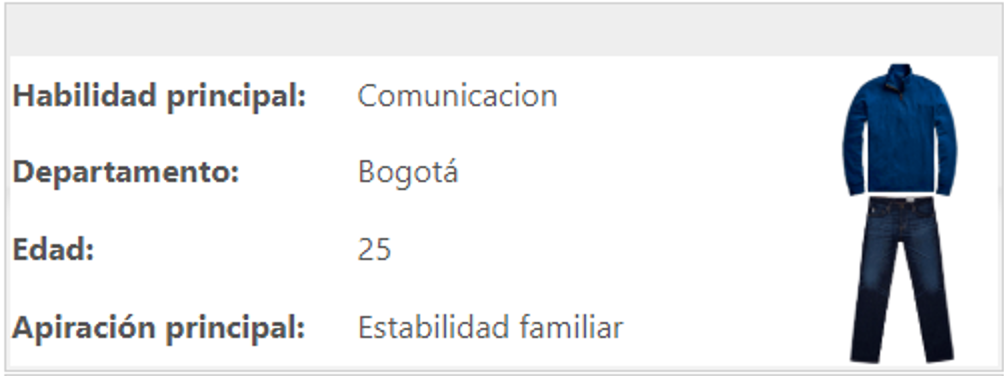
\includegraphics[width=7.7cm]{Images/tarjeta}
	\label{fig:tarjeta}
\end{figure}

